\documentclass[../diplomski_rad.tex]{subfiles}

\begin{document}

\sloppy

\justifying

%uvod u poglavlje
Analiza bioelekričke impedancije je neinvazivna metoda kojom se procjenjuje sastav ljudskog tijela. 
Kroz tijelo se pušta slaba struja te se mjeri pad napona čime se izračunava impedancija tijela. 
Mjerenjem bioimpedancije moguće je praćenje kretanja tekućina kroz tijelo što je vrijedna dijagnostička metoda za praćenje stanja srčanih bolesnika. 

\section{Sastav ljudskog tijela}

Ljudsko tijelo je kompleksna biološka struktura koja se sastoji od različitih međusobno povezanih tkiva koja 
omogućavaju funkcioniranje organizma. Tkiva se približno sastoje od 
64\% vode,
20\% proteina,
10\% masti 
i 5\% minerala. 
Valja napomenuti kako na sastav ljudskog tijela utječu pojedini faktori, kao što su spol i dob \cite{Bera2014}.  

Procjena sastava ljudskog tijela pruža važne informacije koje se koriste u praćenju zdravlja, 
procjeni rizika od pojedinih bolesti, praćenju oporavka te ranom otkrivanju zdravstvenih problema. 

Voda je osnovni element stanica i tkiva te je nužna za brojne fiziološke procese u organizmu, 
kao na primjer održavanje elektrolitske ravnoteže i regulacija temperature.
Ukupnu vodu u tijelu (engl. \textit{Total Body Water; TBW}) 
dijelimo na intracelularnu vodu (engl. \textit{Intracellular Water; ICW}) i ekstracelularnu vodu (engl. \textit{Extracellular Water; ECW}). 
Važni parametri pri analizi ljudskog tijela su i masa tijela bez masnog tkiva (engl. \textit{Fat Free Mass; FFM}) 
te masa masnog tkiva (engl. \textit{Fat Mass; FM}) \cite{Bera2014}.

Ekstracelularna voda je količina vode koja se nalazi izvan stanica te čini 30-40\% ukupne vode. Uključuje krv, limfu, tekućinu u 
zglobovima i međustaničnom prostru. Ima važnu ulogu u transportu kisika i hranjivih tvari do stanica te odvođenju otpadnih 
tvari iz organizma \cite{Bera2014}.

Intracelularna voda je voda koja se nalazi unutar stanica. Ona čini 60-70\% ukupne vode u tijelu. 
Ključna je za mnoge biološke procese unutar stanica, kao na primjer održavanje ravnoteže elektrolita. 
Održavanje ravnoteže između ekstracelularne i intracelularne vode ključno je za normalno funkcioniranje organizma \cite{Bera2014}.

Masno tkivo je također važno za funkcioniranje organizma jer pruža energetsku rezervu, toplinsku izolaciju te štiti unutarnje organe. 
Prekomjerno nakupljanje masnoće može dovesti do različitih zdravstvenih problema, poput pretilosti, dijabetesa i 
bolesti kardiovaskularnog sustava. 
Zbog toga je praćenje udjela masnog tkiva u organizmu važno u procijeni rizika od brojnih bolesti \cite{Bera2014}.

Masu tijela bez masnog tkiva dobijemo tako da od ukupne mase tijela oduzmemo masu masnog tkiva. 
FFW uključuje tjelesnu vodu, mišiće, kosti, organe i druga tkiva osim masnih tkiva te predstavlja masu koja je aktivna i sudjeluje 
u metaboličkim procesima \cite{Bera2014}.

Koliko dobro će tkivo provoditi struju, ovisi o količini vode u njemu. 
Tkiva koja imaju više vode u sebi, kao na primjer mišići, bolje provode eletričnu struju nego masno tkivo koje ne sadrži vodu. 
Zbog toga se sastav ljudskog tijela procjenjuje iz izmjerene bioimpedancije između različitih dijelova tijela. 
Iz bioimpedancije sastav tijela se dobiva putem teorijskih jednadžbi ili tablica koje ovise o parametrima 
kao što su spol, dobna skupina, težina i visina.

\section{Cole model bioimpedancije}

- modeliranje impedeancije

- elektricki model stanice

Matematički model kojim se najčešće modelira bioimpedancija ljudskog tijela naziva se Cole model. 
Razvio ga je britanski fizičar Kenneth Cole 1940-tih godina. 
Cole model opisuje impedanciju tijela kao funkciju frekvencije zbog cega ga koristimo pri analizi sastava ljudskog tijela \cite{Freeborn2021}. 
Orgnialna jednadžba Cole modela glasi: 
\begin{equation}
    \label{jed:drugajednadzba}
    Z(\omega) = R_{\infty}+\frac{R_{0}-R_{\infty}}{1+(j\omega\tau)^{\alpha}} 
\end{equation} 

$R_{\infty}$ prestavlja otpor tkiva na beskonačnoj frekvenciji dok $R_{0}$ prestavlja otpor na nultoj frekvenciji. 
Razlika otpora $R_{\infty}-R_{0}$ prestavlja dodatan otpor struji na niskim frekvencijama zbog nepropusnosti stanične membrane. 
$C_{CPE}$ je element s konstantnom fazom koji modelira kapacitivnost stanične membrane. Njegova impedancija iznosi: 

\begin{equation}
    \label{jed:prvajednadzba}
    Z_{CPE}(\omega) = \frac{1}{(j\omega)^{\alpha}C}
\end{equation} 

Konačno, dobivamo električki model koji je prikazan na slici \ref{slk:cole_model}.
\begin{figure}[htb]
    \centering
    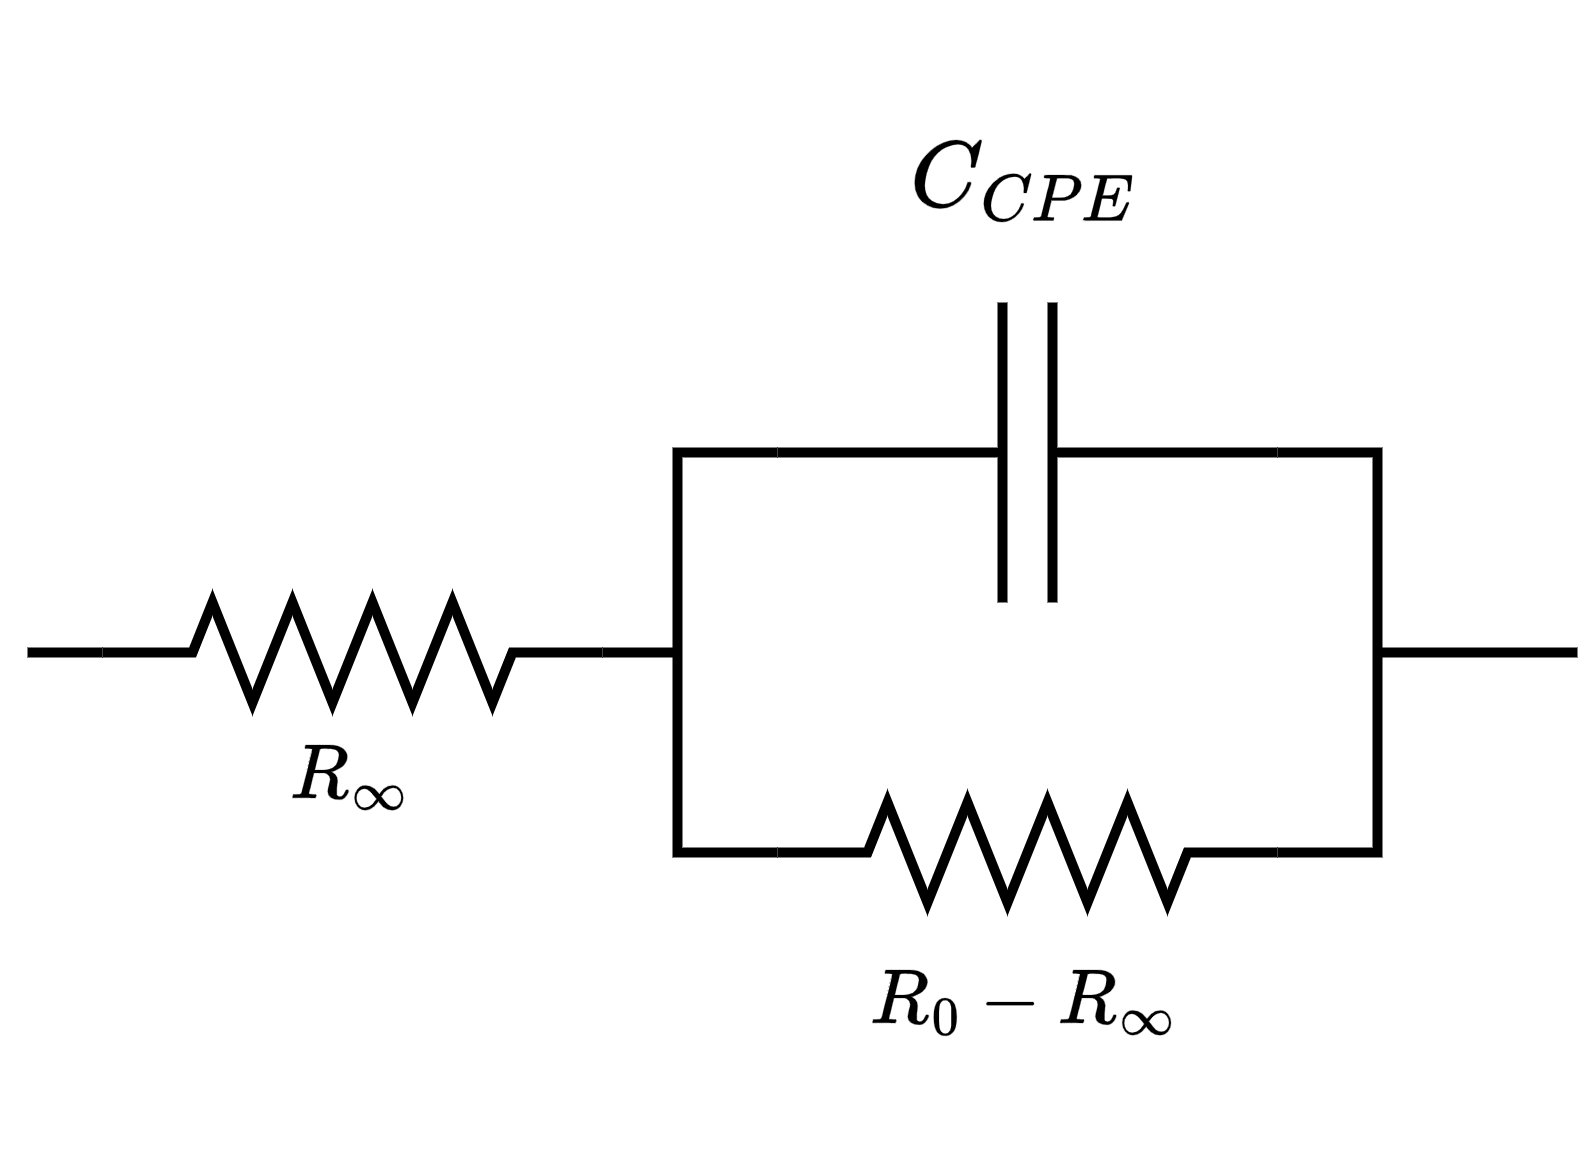
\includegraphics[width=0.6\textwidth]{Figures/cole_model.png} 
    \caption{Cole model bioimpedancije}
    \label{slk:cole_model}
\end{figure}

- opisati Cole graf

\begin{figure}[htb]
    \centering
    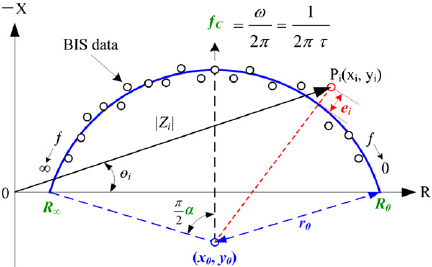
\includegraphics[width=0.7\textwidth]{Figures/cole_plot.png} 
    \caption{Graf bioimpedancije Cole modela \cite{Yang_2013}}
    \label{slk:cole_graf}
\end{figure}

\section{Metode mjerenja bioimpedancije}

Mjerenje bioimpedancije (engl. \textit{Bioelectrical Impedance Analysis; BIA})  djelimo na 
analizu jednom frekvencijom (engl. \textit{Single frequency BIA; SF-BIA}) 
i analizu na više frevencija(engl. \textit{Multi frequency BIA; MF-BIA}). 
Važna metoda je i bioelektrička spektrografija (engl. \textit{Bioelectrical spectroscopy; BIS}) 
koja daje rezultate kroz širok raspon frekvencija. 

SF-BIA je najjednostavnija i najbrža metoda jer koristi samo mjerenje impedancije jednom frekvencijom, najčešće 50 kHz. 
Iz izmjerene bioimpedancije matematičkim izračunima dobivaju se ukupna tjelesna voda, mišićna masa i masa masnog tkiva. 
Ova metoda ima najmanju preciznost jer se podatci prikupljaju na samo jednoj frekvenciji uzbudne struje.

MF-BIA koristi nekoliko različitih frekvencija čime se postiže veća točnost i mogućnst procjene dodatnih parametara, 
kao što su količine intracelularne i ekstracelularne vode. To je moguće jer stanična membrana blokira struju na niskim frekvencijama, 
a propušta ju na višim. 

Bioelektrička spektrografija najpreciznija je metoda mjerenja bioimpedancije. 
Mjerenja se vrše na širokom rasponu frekvencija, od 1 kHz do 1 MHz.  
Ovom metodom možemo procijeniti otpor na nultoj i beskonačnoj frekvenciji, parametre iz Cole modela bioimpedancije 
opisane u prethodnom poglavlju. 
Mjerenje BIS metodomom zbog mnogo frekvencija traje duže i matematički izračuni su kompliciraniji, 
ali pruža  detaljniju i precizniju analizu sastava ljudskog tijela

Postupak mjerenja bioimpedancije svih ranije opisanih metoda je puštanje slabe, 
frekvencijski ovisne izmjenične struje kroz tkivo te mjerenje pada napona. 
Zatim se impedancija izračunava prema:
\begin{equation}
    \label{jed:prvajednadzba}
    Z\angle\theta = \frac{U\angle\theta_{1}}{I\angle\theta_{2}} 
\end{equation} 

Pri mjerenju bioimpedancije razlikujemo dvožično i četverožično spajanje elektroda. 
Kod dvožičnog mjerenja isti par elektroda služi za pobudnu struju i za mjerenje napona. 
Zbog toga dolazi do greške u mjerenju napona uzrokovane padom napona na elektrodama. 
Četverožično mjerenje je preciznije jer se pad napona mjeri direktno na koži i zbog toga će se koristiti u ovom radu \cite{Abasi2022}. 

Važan dio mjernog sustava su i elektrode, koje kroz sučelje koža-elektroda omogućavaju protjecanje struje od mjernog sustava do tkiva. 
U ovom radu usporediti će se rezultati s dvama različitim vrstama elektroda, tradicionalnim metalnim elektrodama te tekstilnim elektrodama. 
Tekstilne elektrode izrađene su od tkanina impregniranih provodnim materijalima, najčešće srebrom. 
Njihova najveća prednost je udobnost i fleksibilnost te mogućnost integracije u odjeću.
Na taj način pacijenti ih neometano mogu nositi tokom svakodnevnih aktivnosti i dužeg vremenskog perioda. 
Međutim, metalne elektrode su manje osjetljive na vanjske parametre kao što su temperatura i oznojenje kože što daje pouzdanije rezultate mjerenja. 
\cite{Meding2021}

Sve opisane metode predstavljaju jednostavan i neizvazivan postupak mjerenja bioimpedancije. 
Važno je napomenuti kako izmjerena impedancija ovisi o brojim faktorima kao što su položaj tijela, hidracija, temperatura tijela i drugi 
što treba uzeti u obzir pri obradi rezultata mjerenja.


\end{document}